\subsection{SkateparksStack}
\subsubsection{SkateparksList}
Auf der ersten Seite sollte man sofort einen Überblick über alle Skateparks erhalten, die wir in
unserer Datenbank gespeichert haben.

\begin{figure}[H]
  \begin{center}
    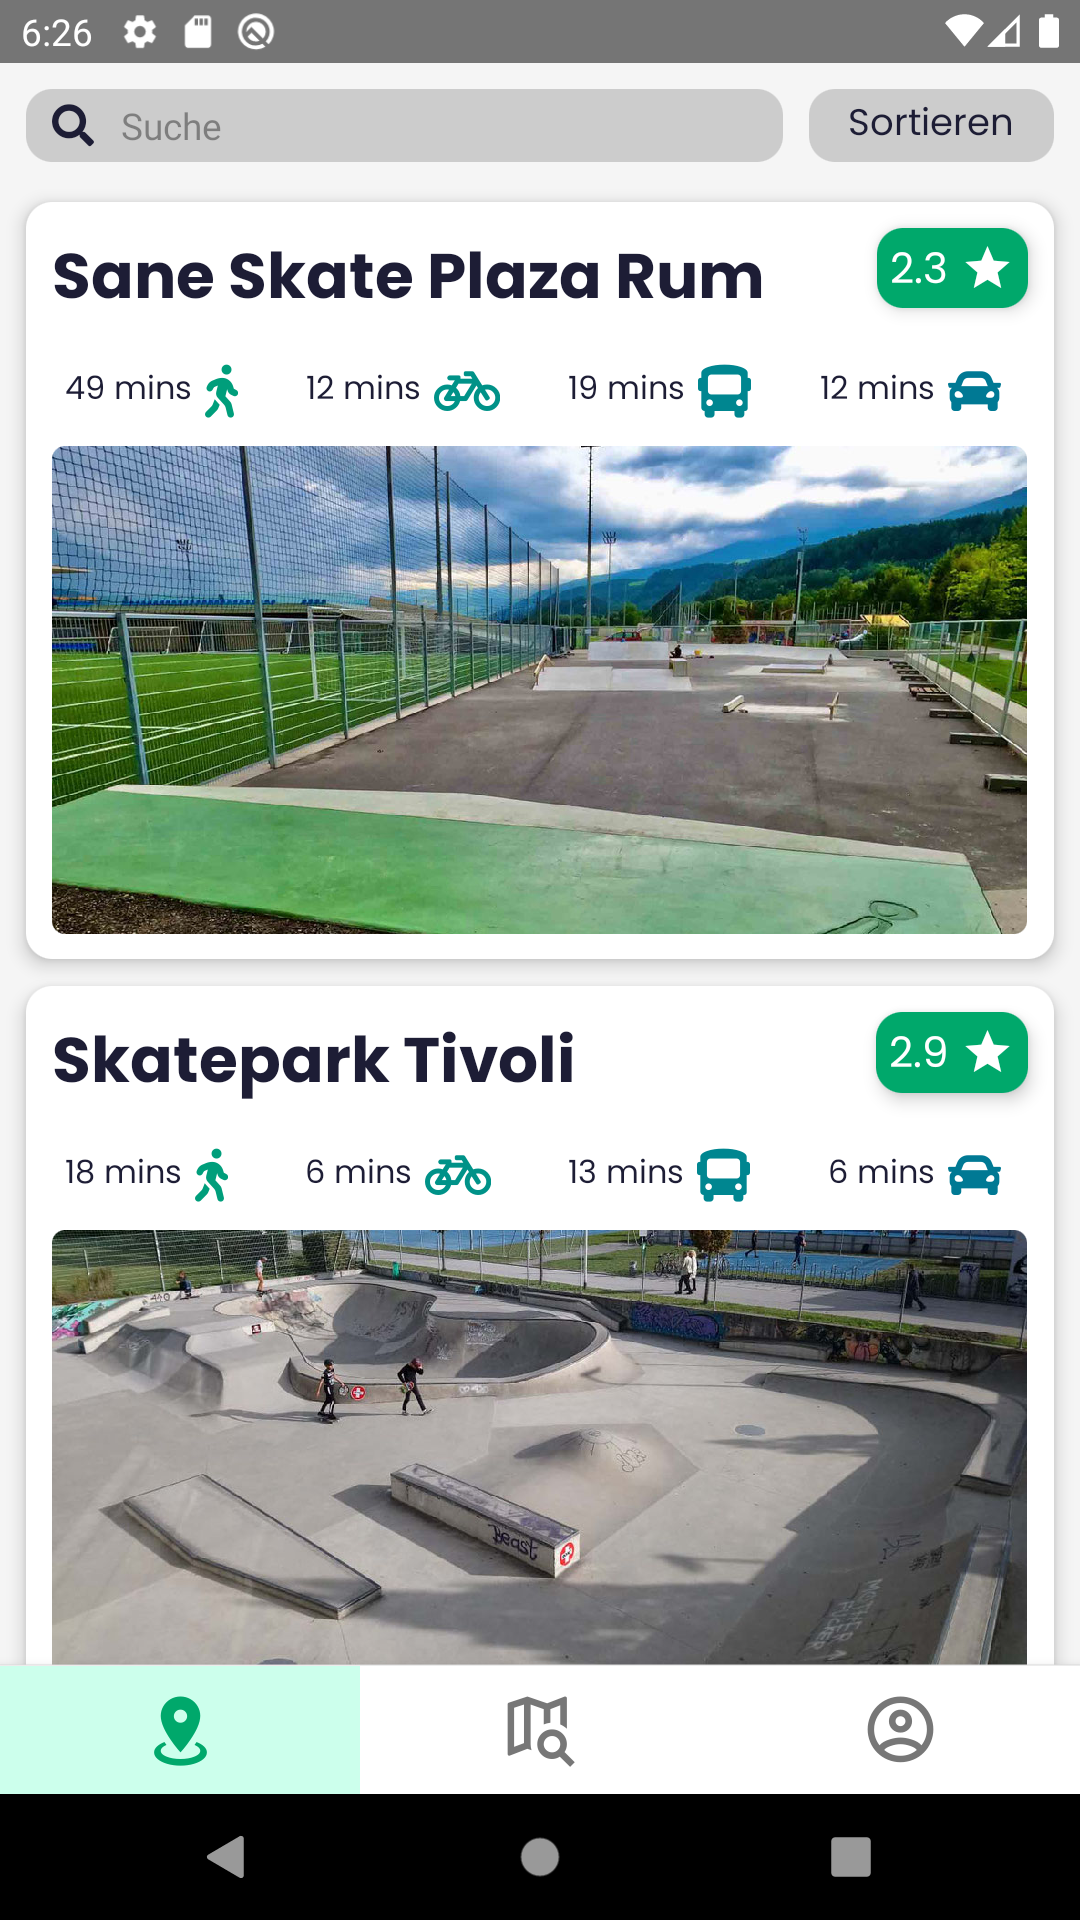
\includegraphics[width=0.6\textwidth]{Mobile/Skateparks/SkateparksList.png}
    \caption{SkateparksList Screen}
  \end{center}
\end{figure}

Wenn der Benutzer auf einen Skatepark drückt, wird bei der Navigation zu SkateparkDetails der
Skatepark übergeben, um die Informationen anzuzeigen.

Am oberen Rand des Bildschirms hat der Benutzer die Möglichkeit, nach einem bestimmten
Skateparknamen zu suchen und nach der Reisezeit zu sortieren, aufsteigend und absteigend.

\begin{figure}[H]
  \begin{center}
    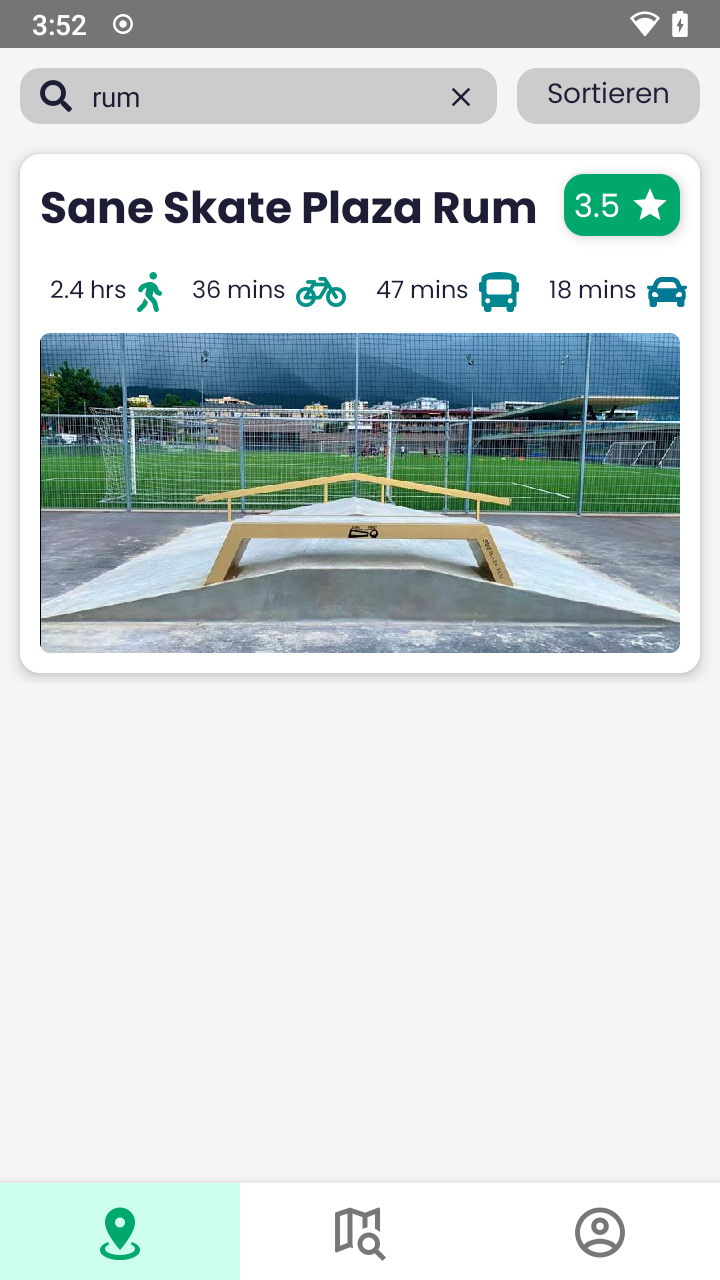
\includegraphics[width=0.6\textwidth]{Mobile/Skateparks/Search.png}
    \caption{Suchfunktion Demonstration}
  \end{center}
\end{figure}

\begin{figure}[H]
  \begin{center}
    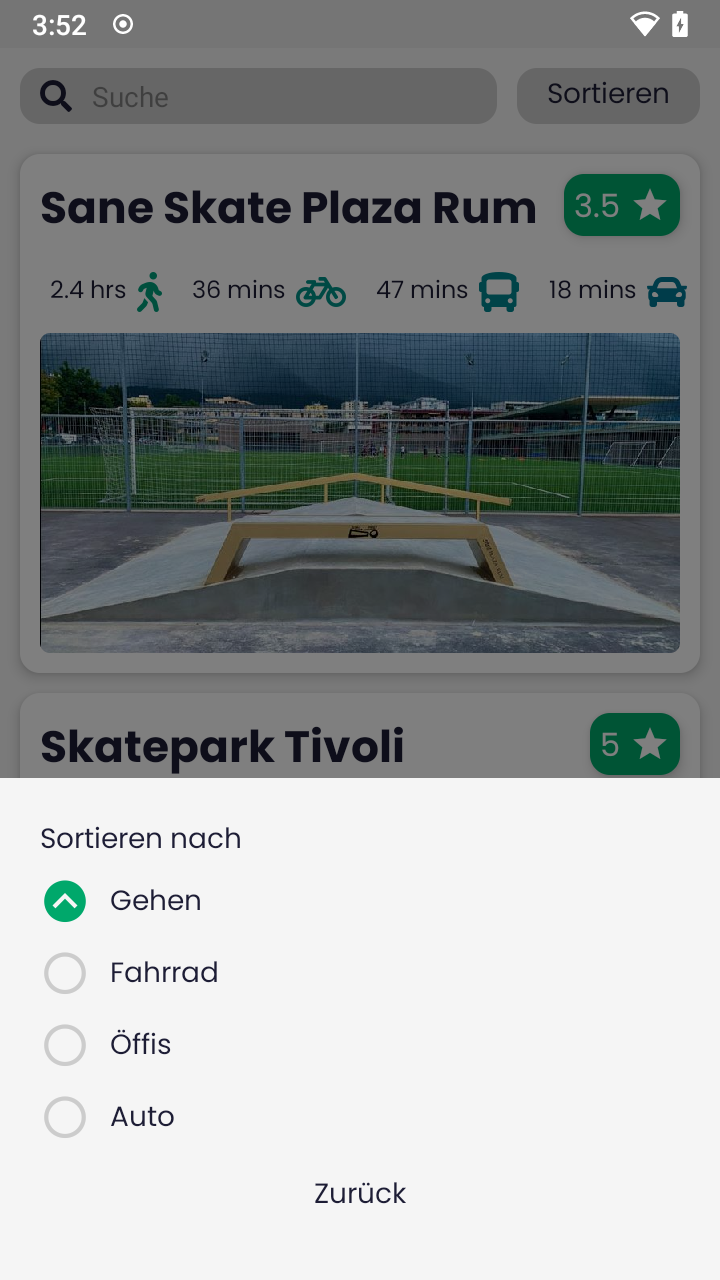
\includegraphics[width=0.6\textwidth]{Mobile/Skateparks/SortModal.png}
    \caption{Sortieren nach Zeit}
  \end{center}
\end{figure}

\newpage

\subsubsection{SkateparkDetails}
Als erstes werden die wichtigsten Informationen zum Standort des Parks angezeigt. Darunter gibt es
eine kleine Diashow mit diversen Bildern des Parks.

\begin{figure}[H]
  \begin{center}
    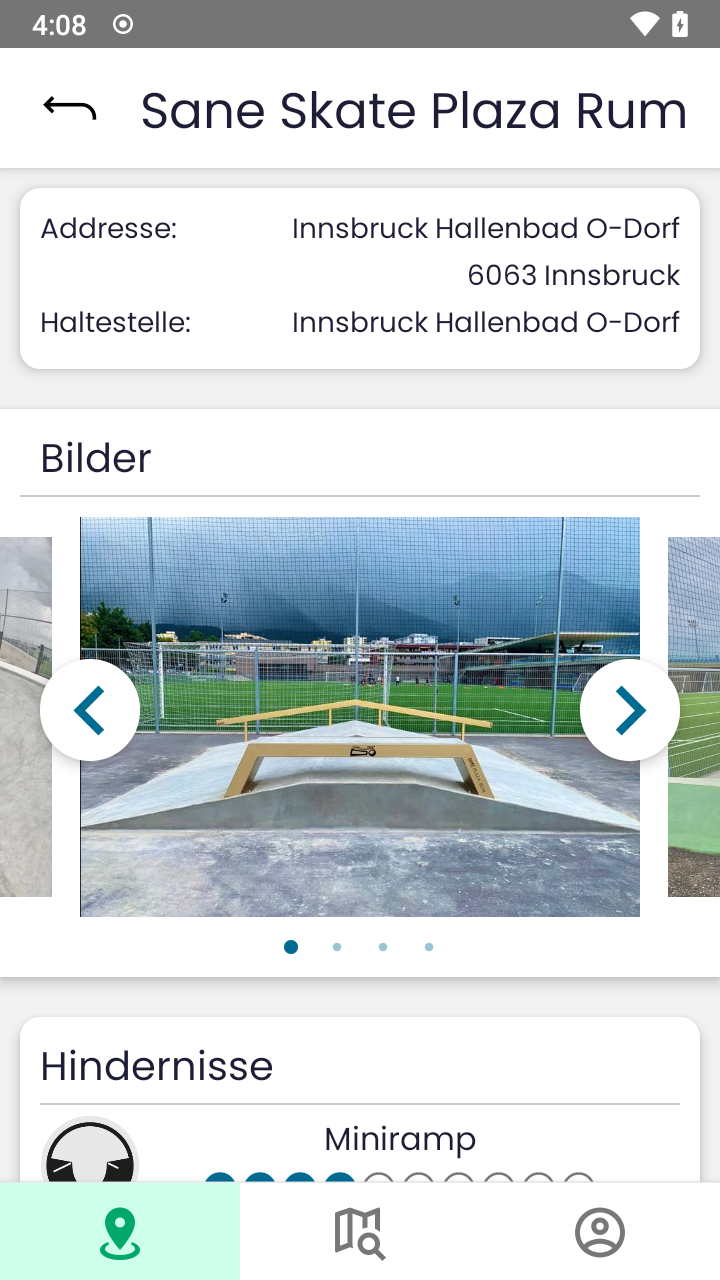
\includegraphics[width=0.6\textwidth]{Mobile/Skateparks/SkateparkDetails.png}
    \caption{Adresse und nächste Haltestelle werden als erstes gezeigt}
  \end{center}
\end{figure}

\begin{figure}[H]
  \begin{center}
    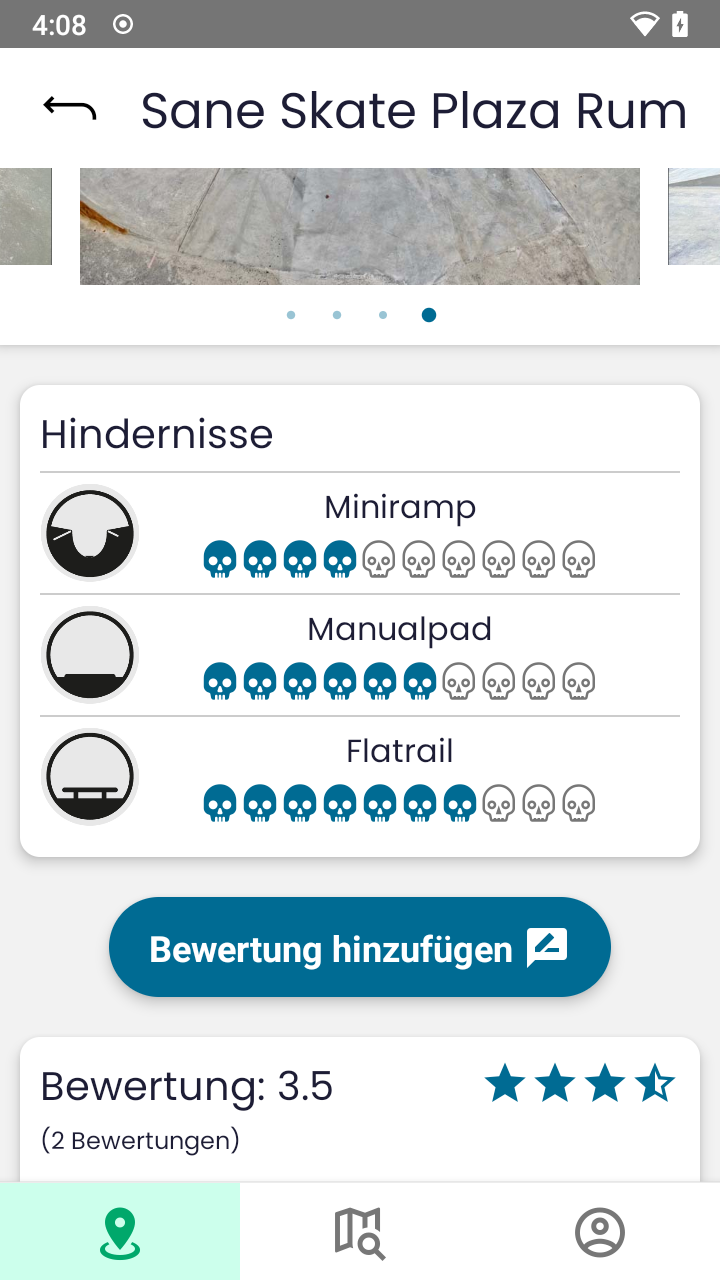
\includegraphics[width=0.6\textwidth]{Mobile/Skateparks/Obstacles.png}
    \caption{Zu jedem Park werden auch Hindernisse mit Schwierigkeitseinschätzungen abgespeichert}
  \end{center}
\end{figure}

Um eine Bewertung zu hinterlassen, drückt der Benutzer auf den Knopf "Bewertung hinzufügen" und
füllt das angezeigte Formular aus. Anschließend werden die Daten an das Backend geschickt und
abgespeichert.

\begin{figure}[H]
  \begin{center}
    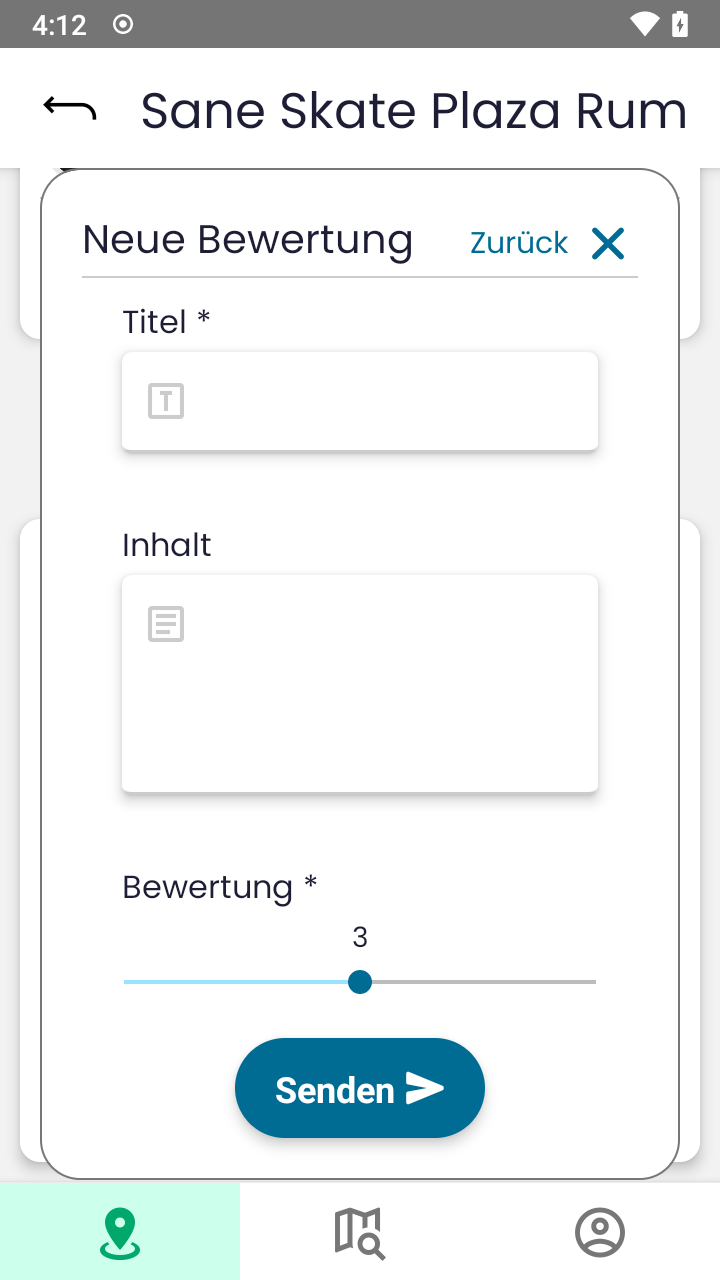
\includegraphics[width=0.6\textwidth]{Mobile/Skateparks/AddReview.png}
    \caption{Daten eintragen und absenden.}
  \end{center}
\end{figure}

Am Ende wird noch die durchschnittliche Bewertung, die Anzahl der Bewertungen und alle Bewertungen
selbst angezeigt.

\begin{figure}[H]
  \begin{center}
    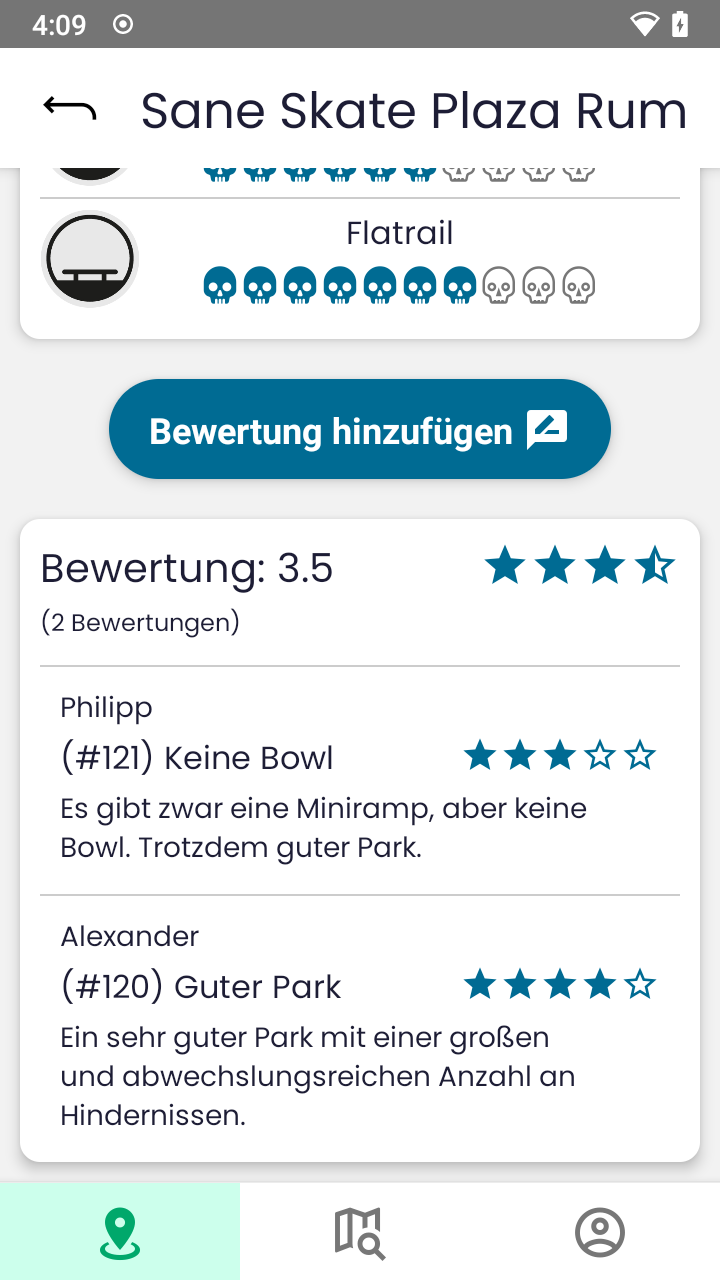
\includegraphics[width=0.6\textwidth]{Mobile/Skateparks/Reviews.png}
    \caption{Alle Bewertungen}
  \end{center}
\end{figure}
